\chapter{Results}\label{chapter-results}
\indent
	\begin{enumerate}
		\item Mean score reaches about \textcolor{blue}{\textbf{77510}} after 350K iterations training (See Figure \ref{result-plot}).
		\begin{figure}[H]
			\centering
			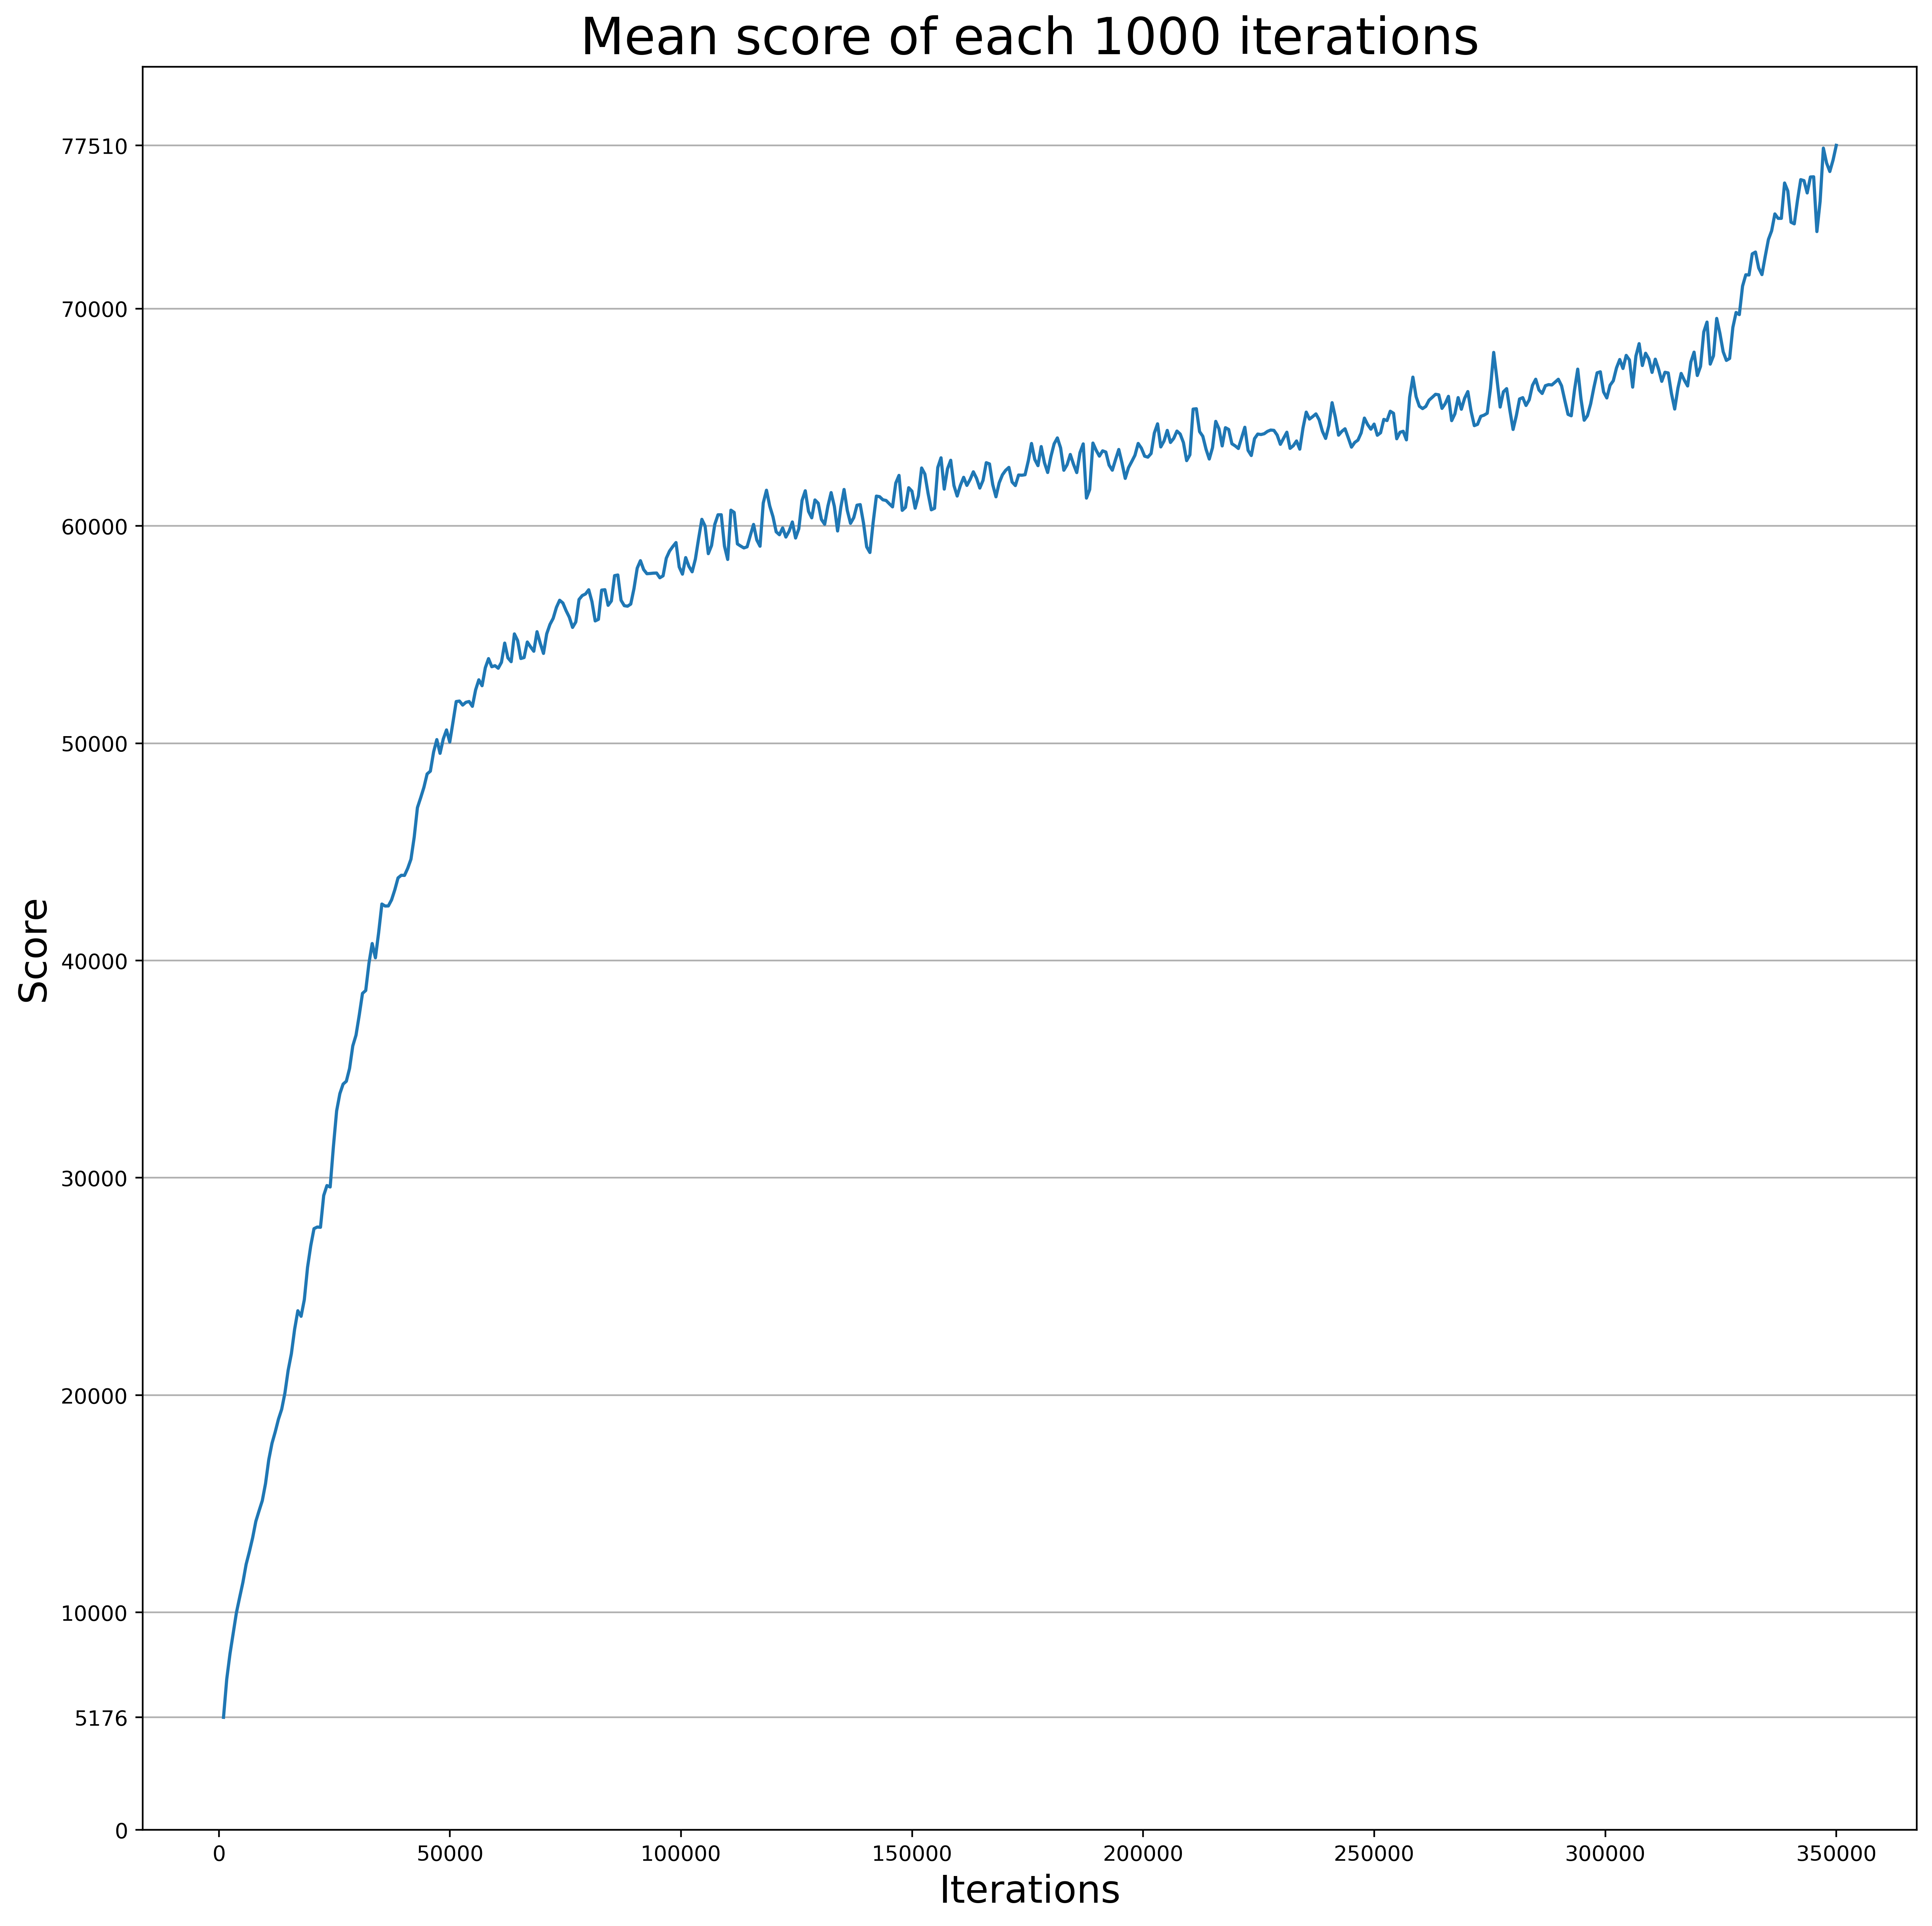
\includegraphics[scale=0.4]{img/result-plot.png}
			\caption{Mean score of each 1K iterations for total 350K iterations.}
			\label{result-plot}
		\end{figure}
		\pagebreak
		\item Average reached 2048-tile percentage is about \textcolor{blue}{\textbf{95\%}} after 350K iterations training (See Figure \ref{result-print}).
		\begin{figure}[H]
			\centering
			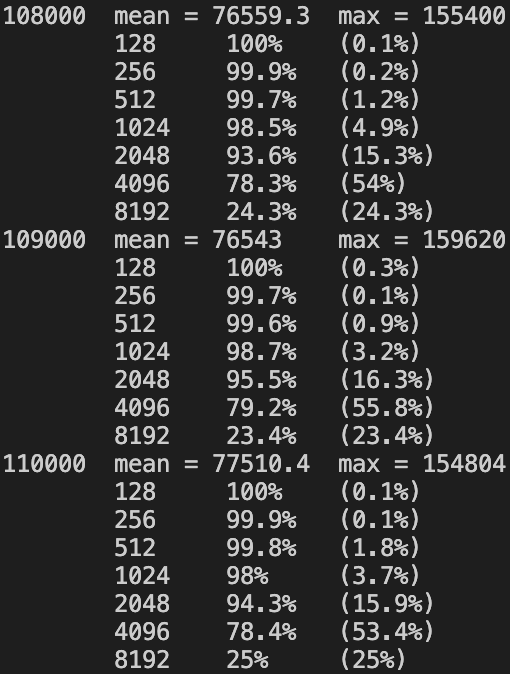
\includegraphics[scale=0.6]{img/result-print.png}
			\caption{Score details after 350K training.\protect\footnotemark}
			\label{result-print}
		\end{figure}
		\footnotetext{Note that the printed iterations here are wrong, since the model is trained 240K iterations at first and stop, then 
		load the weight, and trained for 110K iterations for the second time. Totally 350K iterations training.}
	\end{enumerate}
